\documentclass[a4paper,12pt]{ltjsarticle}

% LuaLaTeX用パッケージ
\usepackage{luatexja}
\usepackage{luatexja-fontspec}
\usepackage{amsmath,amssymb,amsthm}
\usepackage{tikz}
\usetikzlibrary{arrows,positioning,calc,shapes}
\usepackage{listings}
\usepackage{hyperref}
\usepackage{xcolor}

% 定理環境
\theoremstyle{definition}
\newtheorem{definition}{定義}[section]
\newtheorem{theorem}[definition]{定理}
\newtheorem{lemma}[definition]{補題}
\newtheorem{proposition}[definition]{命題}
\newtheorem{example}[definition]{例}
\newtheorem{remark}[definition]{注意}

% Leanコード用設定
\lstdefinelanguage{Lean}{
  keywords={def,theorem,lemma,structure,where,namespace,end,import,abbrev,instance,open,section},
  keywordstyle=\color{blue}\bfseries,
  commentstyle=\color{green!60!black},
  morecomment=[l]{--},
  morecomment=[s]{/-}{-/},
  basicstyle=\ttfamily\small,
  breaklines=true,
  showstringspaces=false
}

\title{算法的マルチンゲール理論の形式化\\
  {\large 離散有限標本空間上の構造塔的アプローチ}}
\author{生成：Claude Code (Anthropic) \\
  Lean形式化：CODEX (OpenAI)}
\date{\today}

\begin{document}

\maketitle

\begin{abstract}
本稿では、離散有限標本空間上のマルチンゲール理論を構造塔（Structure Tower）の枠組みで形式化する。具体的には、決定可能な事象、有限代数、離散フィルトレーション、計算可能な停止時間を段階的に構築し、最終的にOptional Stopping Theorem（任意停止定理）の計算可能版を与える。すべての構成は型理論的に検証可能であり、\texttt{\#eval}による具体的な計算が可能である。
\end{abstract}

\tableofcontents

\section{序論}

本稿の目的は、確率論におけるマルチンゲール理論を、有限標本空間上で\emph{計算可能}かつ\emph{形式的に検証可能}な形で構築することである。従来の測度論的アプローチとは異なり、ここでは以下の特徴を持つ：

\begin{itemize}
\item \textbf{有限性}：標本空間は常に有限集合
\item \textbf{決定可能性}：すべての事象のメンバーシップ判定が計算可能
\item \textbf{構造塔}：フィルトレーションを構造塔の具体例として扱う
\item \textbf{形式化}：Lean 4で完全に形式化
\end{itemize}

\subsection{階層構造}

本稿で扱う理論は、以下の7層からなる階層構造を持つ：

\begin{center}
\begin{tikzpicture}[node distance=1.5cm, auto]
  \node (tower) [rectangle, draw, fill=blue!20, text width=6cm, align=center]
    {構造塔の例\\DecidableStructureTower\_Examples};
  \node (events) [rectangle, draw, fill=green!20, text width=6cm, align=center, below of=tower]
    {決定可能事象\\DecidableEvents};
  \node (algebra) [rectangle, draw, fill=green!20, text width=6cm, align=center, below of=events]
    {有限代数\\DecidableAlgebra};
  \node (filtration) [rectangle, draw, fill=yellow!20, text width=6cm, align=center, below of=algebra]
    {離散フィルトレーション\\DecidableFiltration};
  \node (stopping) [rectangle, draw, fill=yellow!20, text width=6cm, align=center, below of=filtration]
    {計算可能停止時間\\ComputableStoppingTime};
  \node (core) [rectangle, draw, fill=orange!20, text width=6cm, align=center, below of=stopping]
    {マルチンゲール基礎\\AlgorithmicMartingaleCore};
  \node (ost) [rectangle, draw, fill=red!20, text width=6cm, align=center, below of=core]
    {任意停止定理\\AlgorithmicMartingale\_v0};

  \draw[->] (tower) -- (events);
  \draw[->] (events) -- (algebra);
  \draw[->] (algebra) -- (filtration);
  \draw[->] (filtration) -- (stopping);
  \draw[->] (stopping) -- (core);
  \draw[->] (core) -- (ost);
\end{tikzpicture}
\end{center}

\section{構造塔の例}

\subsection{構造塔の定義}

\begin{definition}[構造塔]
構造塔（Structure Tower with Minimal Layer）とは、以下のデータからなる：
\begin{itemize}
\item 台集合 $\mathcal{C}$（carrier）
\item インデックス集合 $I$（前順序付き）
\item 各インデックス $i \in I$ に対する層 $\text{layer}(i) \subseteq \mathcal{C}$
\item 被覆条件：$\forall x \in \mathcal{C}, \exists i \in I, x \in \text{layer}(i)$
\item 単調性：$i \leq j \Rightarrow \text{layer}(i) \subseteq \text{layer}(j)$
\item 最小層関数 $\text{minLayer} : \mathcal{C} \to I$ であって、
  \begin{itemize}
  \item $x \in \text{layer}(\text{minLayer}(x))$（健全性）
  \item $x \in \text{layer}(i) \Rightarrow \text{minLayer}(x) \leq i$（最小性）
  \end{itemize}
\end{itemize}
\end{definition}

\subsection{具体例：整数塔}

整数を絶対値で層別化した構造塔：

\begin{example}[整数の絶対値塔]
$\mathcal{C} = \mathbb{Z}$, $I = \mathbb{N}$として、
\[
\text{layer}(n) = \{k \in \mathbb{Z} \mid |k| \leq n\}
\]
と定義すると、
\[
\text{minLayer}(k) = |k|
\]
が最小層関数となる。
\end{example}

\begin{center}
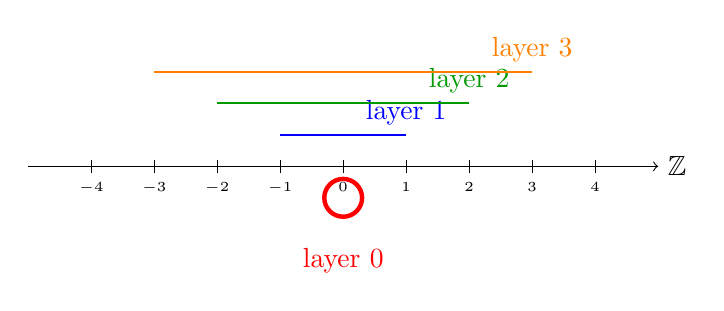
\begin{tikzpicture}[scale=0.8]
  \draw[->] (-5,0) -- (5,0) node[right] {$\mathbb{Z}$};
  \foreach \x in {-4,-3,-2,-1,0,1,2,3,4}
    \draw (\x,0.1) -- (\x,-0.1) node[below] {\tiny $\x$};

  % layer 0
  \draw[red, ultra thick] (0,-0.5) circle (0.3cm) node[below=0.5cm] {layer 0};
  % layer 1
  \draw[blue, thick] (-1,0.5) -- (1,0.5) node[above] {layer 1};
  % layer 2
  \draw[green!60!black, thick] (-2,1) -- (2,1) node[above] {layer 2};
  % layer 3
  \draw[orange, thick] (-3,1.5) -- (3,1.5) node[above] {layer 3};
\end{tikzpicture}
\end{center}

\subsection{具体例：リスト塔、多項式塔}

同様に、リストを長さで、多項式を次数で層別化できる：
\begin{itemize}
\item \textbf{リスト塔}：$\text{layer}(n) = \{l \mid \text{length}(l) \leq n\}$
\item \textbf{多項式塔}：$\text{layer}(n) = \{p \mid \deg(p) \leq n\}$
\end{itemize}

\section{決定可能事象}

\subsection{有限標本空間}

\begin{definition}[有限標本空間]
有限標本空間とは、型 $\Omega$ であって以下を満たすもの：
\begin{itemize}
\item \texttt{Fintype $\Omega$}：$\Omega$は有限型
\item \texttt{DecidableEq $\Omega$}：等号判定が決定可能
\end{itemize}
\end{definition}

\begin{remark}
有限性により、すべての事象のメンバーシップ判定が決定可能となる。これは無限標本空間との本質的な違いである。
\end{remark}

\subsection{事象の定義}

\begin{definition}[事象]
標本空間 $\Omega$ 上の事象とは、$\Omega$ の部分集合 $A \subseteq \Omega$ である。
\end{definition}

\subsection{基本演算}

事象の基本演算は以下の通り：
\begin{align*}
\text{空事象} &: \emptyset \\
\text{全事象} &: \Omega \\
\text{補集合} &: A^c = \Omega \setminus A \\
\text{和} &: A \cup B \\
\text{積} &: A \cap B
\end{align*}

すべての演算について決定可能性が保証される：

\begin{theorem}[演算の決定可能性]
$\Omega$が有限標本空間で、$A, B$が決定可能事象なら、
$A^c, A \cup B, A \cap B$ もすべて決定可能。
\end{theorem}

\begin{center}
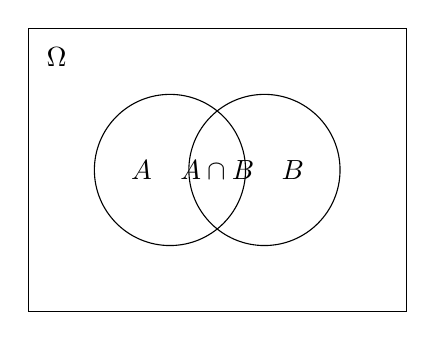
\begin{tikzpicture}[scale=1.2]
  \draw (0,0) rectangle (4,3);
  \draw (1.5,1.5) circle (0.8cm);
  \draw (2.5,1.5) circle (0.8cm);
  \node at (1.2,1.5) {$A$};
  \node at (2.8,1.5) {$B$};
  \node at (0.3,2.7) {$\Omega$};
  \node at (2,1.5) {$A \cap B$};
\end{tikzpicture}
\end{center}

\section{有限代数}

\subsection{定義と性質}

\begin{definition}[有限代数]
標本空間 $\Omega$ 上の有限代数 $\mathcal{F}$ とは、事象の族であって以下を満たすもの：
\begin{enumerate}
\item $\emptyset \in \mathcal{F}$（空事象を含む）
\item $A \in \mathcal{F} \Rightarrow A^c \in \mathcal{F}$（補集合で閉じる）
\item $A, B \in \mathcal{F} \Rightarrow A \cup B \in \mathcal{F}$（和で閉じる）
\end{enumerate}
\end{definition}

\begin{remark}
これは $\sigma$-代数の有限版である。有限標本空間では、すべての有限代数は $\sigma$-代数となる。
\end{remark}

\begin{proposition}[派生性質]
有限代数 $\mathcal{F}$ について以下が成り立つ：
\begin{enumerate}
\item $\Omega \in \mathcal{F}$（全事象を含む）
\item $A, B \in \mathcal{F} \Rightarrow A \cap B \in \mathcal{F}$（積で閉じる）
\item $A, B \in \mathcal{F} \Rightarrow A \setminus B \in \mathcal{F}$（差で閉じる）
\end{enumerate}
\end{proposition}

\subsection{具体例}

\begin{example}[自明な代数]
$\mathcal{F} = \{\emptyset, \Omega\}$ は最小の有限代数である。
\end{example}

\begin{example}[サイコロの偶奇代数]
サイコロの標本空間 $\Omega = \{1,2,3,4,5,6\}$ に対し、
\[
\mathcal{F} = \{\emptyset, \{2,4,6\}, \{1,3,5\}, \Omega\}
\]
は有限代数をなす。これは「偶数か奇数か」という情報のみを表現する。
\end{example}

\section{離散フィルトレーション}

\subsection{フィルトレーションの定義}

\begin{definition}[離散フィルトレーション]
有限標本空間 $\Omega$ 上の離散フィルトレーションとは、以下のデータからなる：
\begin{itemize}
\item 時間地平 $N \in \mathbb{N}$（timeHorizon）
\item 各時刻 $t \leq N$ に対する有限代数 $\mathcal{F}_t$
\item 単調性：$s \leq t \Rightarrow \mathcal{F}_s \subseteq \mathcal{F}_t$
\end{itemize}
\end{definition}

単調性は「情報の増加」を表す：時間が進むにつれ、観測可能な事象が増える。

\begin{center}
\begin{tikzpicture}[node distance=2cm]
  \node (F0) [circle, draw] {$\mathcal{F}_0$};
  \node (F1) [circle, draw, right of=F0] {$\mathcal{F}_1$};
  \node (F2) [circle, draw, right of=F1] {$\mathcal{F}_2$};
  \node (Fn) [circle, draw, right of=F2] {$\mathcal{F}_N$};
  \node (dots) [right of=F2, xshift=-1cm] {$\cdots$};

  \draw[->] (F0) -- (F1) node[midway, above] {$\subseteq$};
  \draw[->] (F1) -- (F2) node[midway, above] {$\subseteq$};
  \draw[->] (F2) -- (dots);
  \draw[->] (dots) -- (Fn) node[midway, above] {$\subseteq$};

  \node[below of=F0, yshift=0.5cm] {時刻0};
  \node[below of=F1, yshift=0.5cm] {時刻1};
  \node[below of=F2, yshift=0.5cm] {時刻2};
  \node[below of=Fn, yshift=0.5cm] {時刻$N$};
\end{tikzpicture}
\end{center}

\subsection{構造塔としてのフィルトレーション}

フィルトレーションは構造塔の具体例とみなせる：

\begin{proposition}[フィルトレーションと構造塔]
離散フィルトレーション $(\mathcal{F}_t)_{t=0}^N$ に対し、以下を定義すると構造塔となる：
\begin{itemize}
\item 台集合：事象の全体 $\mathcal{C} = \mathcal{P}(\Omega)$
\item インデックス：時刻 $I = \{0,1,\ldots,N\}$
\item 層：$\text{layer}(t) = \mathcal{F}_t$
\item 最小層：$\text{minLayer}(A) = \min\{t \mid A \in \mathcal{F}_t\}$
\end{itemize}
\end{proposition}

\section{計算可能な停止時間}

\subsection{停止時間の定義}

\begin{definition}[停止時間]
フィルトレーション $(\mathcal{F}_t)$ に対し、確率変数 $\tau : \Omega \to \mathbb{N}$ が停止時間であるとは、
\[
\forall t \leq N, \quad \{\omega \mid \tau(\omega) \leq t\} \in \mathcal{F}_t
\]
が成り立つことである。
\end{definition}

\begin{remark}
停止時間の条件は「$\tau \leq t$ かどうかは時刻 $t$ で判定可能」と解釈できる。これは「未来を見ない」という条件に対応する。
\end{remark}

\subsection{停止時間の演算}

\begin{proposition}[停止時間の最小・最大]
$\tau_1, \tau_2$ が停止時間なら、$\min(\tau_1, \tau_2)$ と $\max(\tau_1, \tau_2)$ も停止時間である。
\end{proposition}

\begin{proof}[証明のスケッチ]
最小の場合：
\[
\{\min(\tau_1, \tau_2) \leq t\} = \{\tau_1 \leq t\} \cup \{\tau_2 \leq t\} \in \mathcal{F}_t
\]
最大の場合：
\[
\{\max(\tau_1, \tau_2) \leq t\} = \{\tau_1 \leq t\} \cap \{\tau_2 \leq t\} \in \mathcal{F}_t
\]
\end{proof}

\begin{center}
\begin{tikzpicture}[scale=0.8]
  \draw[->] (0,0) -- (6,0) node[right] {$\omega$};
  \draw[->] (0,0) -- (0,4) node[above] {時刻};

  \draw[blue, thick] plot coordinates {(0.5,1) (1.5,2) (2.5,1.5) (3.5,3) (4.5,2) (5.5,1)};
  \draw[red, thick] plot coordinates {(0.5,0.5) (1.5,1) (2.5,2.5) (3.5,2) (4.5,3) (5.5,2.5)};

  \node[blue] at (5.5,0.5) {$\tau_1$};
  \node[red] at (0.5,3.5) {$\tau_2$};
  \node[green!60!black] at (3,3.5) {$\min(\tau_1,\tau_2)$};
\end{tikzpicture}
\end{center}

\section{マルチンゲール基礎}

\subsection{確率質量関数}

\begin{definition}[確率質量関数]
有限標本空間 $\Omega$ 上の確率質量関数とは、写像 $P : \Omega \to \mathbb{Q}$ であって、
\begin{enumerate}
\item $\forall \omega, P(\omega) \geq 0$（非負性）
\item $\sum_{\omega \in \Omega} P(\omega) = 1$（全確率）
\end{enumerate}
を満たすものである。
\end{definition}

\subsection{期待値}

\begin{definition}[期待値]
確率変数 $X : \Omega \to \mathbb{Q}$ の期待値は、
\[
\mathbb{E}[X] = \sum_{\omega \in \Omega} P(\omega) \cdot X(\omega)
\]
と定義される。
\end{definition}

\begin{proposition}[期待値の線形性]
\begin{enumerate}
\item $\mathbb{E}[c] = c$（定数の期待値）
\item $\mathbb{E}[aX + bY] = a\mathbb{E}[X] + b\mathbb{E}[Y]$（線形性）
\end{enumerate}
\end{proposition}

\subsection{簡略版マルチンゲール}

\begin{definition}[マルチンゲール（簡略版）]
確率過程 $(M_n)_{n=0}^N$ がマルチンゲールであるとは、
\[
\forall n < N, \quad \mathbb{E}[M_{n+1}] = \mathbb{E}[M_n]
\]
が成り立つことである。
\end{definition}

\begin{remark}
これは条件付き期待値を用いた完全な定義の簡略版である。完全版では $\mathbb{E}[M_{n+1} \mid \mathcal{F}_n] = M_n$ が要求される。
\end{remark}

\section{Optional Stopping Theorem}

\subsection{打ち切り過程}

\begin{definition}[打ち切り過程]
マルチンゲール $(M_n)$ と停止時間 $\tau$ に対し、打ち切り過程 $M^\tau$ を
\[
M^\tau_n(\omega) = M_{\min(n, \tau(\omega))}(\omega)
\]
と定義する。
\end{definition}

\subsection{Optional Stopping Theorem}

\begin{theorem}[Optional Stopping Theorem（有界版）]
$(M_n)_{n=0}^N$ を強マルチンゲールとし、$\tau$ を有界停止時間（$\tau \leq N$）とする。このとき、
\[
\mathbb{E}[M_\tau] = \mathbb{E}[M_0]
\]
が成り立つ。
\end{theorem}

\begin{proof}[証明のアイデア]
テレスコープ分解を用いる：
\begin{align*}
M_\tau - M_0 &= \sum_{n=0}^{N-1} (M_{n+1} - M_n) \cdot \mathbb{1}_{\{\tau > n\}}
\end{align*}
強マルチンゲール性より、各項の期待値は0となる：
\[
\mathbb{E}[(M_{n+1} - M_n) \cdot \mathbb{1}_{\{\tau > n\}}] = 0
\]
なぜなら $\{\tau > n\} \in \mathcal{F}_n$ であり、
\[
\mathbb{E}[M_{n+1} \cdot \mathbb{1}_A] = \mathbb{E}[M_n \cdot \mathbb{1}_A], \quad \forall A \in \mathcal{F}_n
\]
が成り立つからである。
\end{proof}

\subsection{計算例}

定数マルチンゲール $M_n \equiv c$ に対して、任意の停止時間 $\tau$ で
\[
\mathbb{E}[M_\tau] = c = \mathbb{E}[M_0]
\]
が成り立つ。これは自明だが、形式検証においては非自明な定理である。

\section{形式化の意義}

\subsection{計算可能性}

本形式化の最大の特徴は、すべての構成が \texttt{\#eval} で計算可能な点である：

\begin{lstlisting}[language=Lean]
#eval coinConst1.time true   -- 1
#eval coinHeadTail.time true  -- 0
#eval coinMin.time false      -- 1
\end{lstlisting}

\subsection{型理論的検証}

型システムにより以下が保証される：
\begin{itemize}
\item 停止時間の条件は構成的に検証可能
\item マルチンゲール性は型で表現される
\item Optional Stopping Theoremは証明付き定理
\end{itemize}

\section{結論}

本稿では、離散有限標本空間上のマルチンゲール理論を構造塔の枠組みで形式化した。重要な成果は以下の通り：

\begin{enumerate}
\item 決定可能な事象から始め、段階的に理論を構築
\item フィルトレーションを構造塔の具体例として理解
\item 停止時間を情報構造として特徴付け
\item Optional Stopping Theoremの計算可能版を証明
\end{enumerate}

今後の展開としては：
\begin{itemize}
\item 条件付き期待値の完全な実装
\item より一般的なマルチンゲール不等式
\item 確率過程の極限理論への拡張
\end{itemize}

\vspace{1cm}

\noindent \textbf{謝辞}：本文書はClaude Code（Anthropic）により生成され、形式化はCODEX（OpenAI）により実装されました。

\begin{thebibliography}{9}
\bibitem{williams} David Williams, \textit{Probability with Martingales}, Cambridge University Press, 1991.
\bibitem{billingsley} Patrick Billingsley, \textit{Probability and Measure}, Wiley, 1995.
\bibitem{lean} The mathlib Community, \textit{The Lean Mathematical Library}, 2024.
\end{thebibliography}

\end{document}
